\documentclass[10pt]{article}
\usepackage[usenames]{color} %used for font color
\usepackage{amssymb} %maths
\usepackage{amsmath} %maths
\usepackage[utf8]{inputenc} %useful to type directly diacritic characters
\usepackage[letterpaper, portrait, margin=1in]{geometry}
\usepackage{graphicx,wrapfig}
\begin{document}
\subsection*{MSDS610 Week 4 Hive Assignment - Nathan Worsham}
\subsection*{Installing Hive}
Again on this week's assignment I started by powering up my VM from week 1. Since the rest of the software on this VM is installed at /home/hadoop I decided to make the Hive installation location no different and unpacked the archive there along with changing ownership of the files. 
\par
\raisebox{-.6\height}{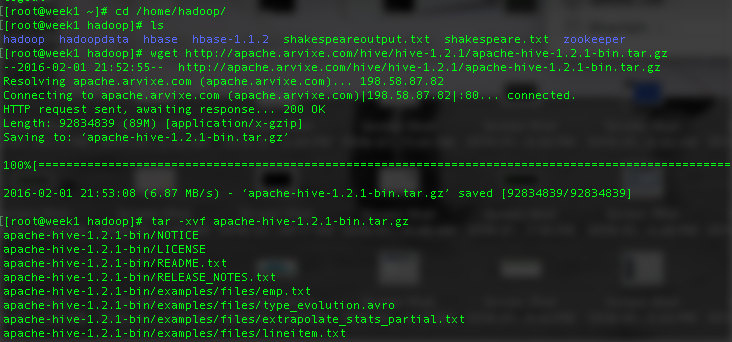
\includegraphics[width=8cm]{get.png}}%
\hfill
\raisebox{-.6\height}{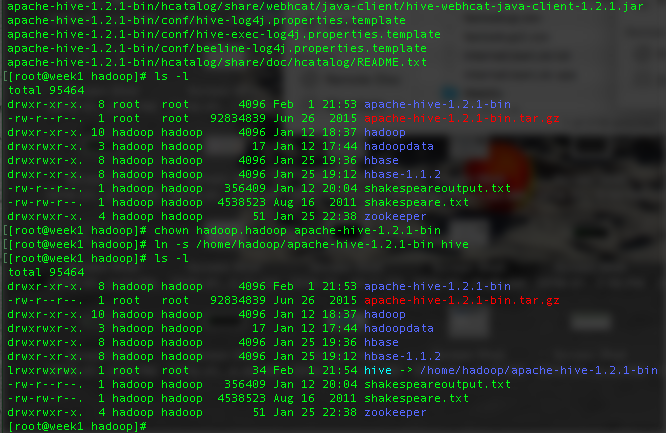
\includegraphics[width=8cm]{chown.png}}%
\par
Next I configured the environment variables to inlude HIVE\_HOME as instructed.
\begin{figure}[!h]
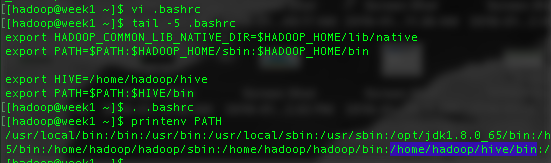
\includegraphics[scale=0.37]{printenv.png}
\centering
\end{figure}\\
\indent Now the instructions wanted directories and permissions established on such directories within the HDFS. Not realizing, I tried making the /tmp directory only to find one already there. It seemed the rights were already correct but equally did not seem it would hurt to make sure with the \verb|chmod| command. When I tried to create layers of directories with the command they provided--\verb|hadoop fs -mkdir /user/hive/warehouse|--it complained of "No such file or directory". Adding the \verb|-p| option like the normal \verb|mkdir| command to "Create intermediate directories as required" worked in the HDFS. I then added the rights to the new directory as well. 
\begin{figure}[!h]
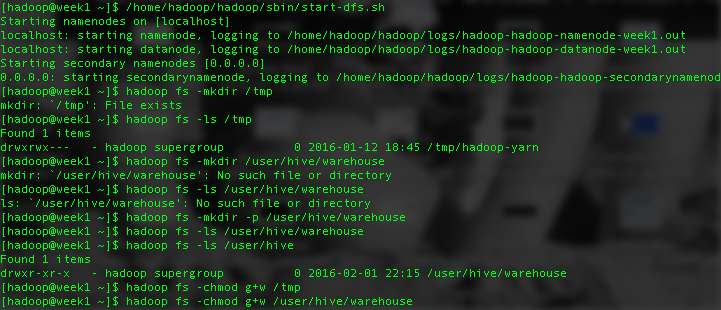
\includegraphics[scale=0.37]{hdfs_create.png}
\centering
\end{figure}\\
\indent I was now ready to start hive, which started up fine. The instructions indicate that HiveCLI is deprecated and that instead "HiveServer2 and Beeline" should be used in it's place. When I tried the first command \verb|$HIVE_HOME/bin/hiveserver2| the shell did not come back, it seems this command starts up a process. I used CTRL-Z to stop it after CTRL-C could not break it. Reading further it seems the instructions offer a single command to run both--\verb|$HIVE_HOME/bin/beeline -u jdbc:hive2://|--but when I ran it I received errors about "initialising [sic] the database". 
\pagebreak
\begin{figure}[!h]
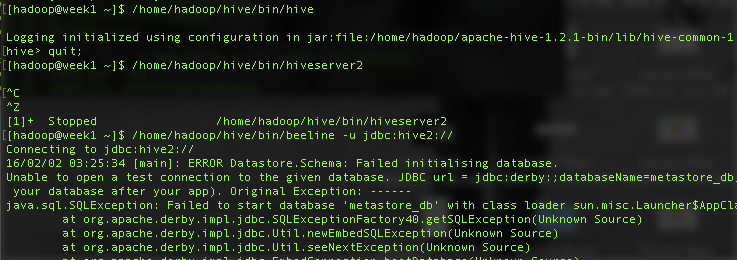
\includegraphics[scale=0.37]{cli_w_error.png}
\centering
\end{figure}\\
\indent Thinking that when I killed the previous command there was likely some fallout, so I rebooted the VM and tried the command again, this time I was received a new error about not being able to create a directory in /tmp inside the HDFS.
\begin{figure}[!h]
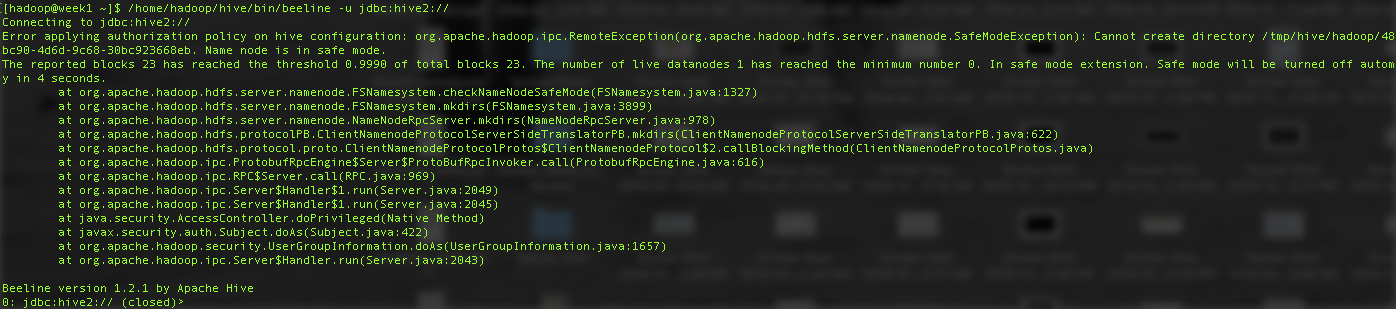
\includegraphics[scale=0.37]{cli_w_error2.png}
\centering
\end{figure}\\
\indent It would seem that similarly to the instruction using the \verb|mkdir| command, the \verb|chmod| command instructions did not account for recursive actions. This is because when I did a file listing in the HDFS of \verb|/tmp/hive| I found that the group portion of the permissions was lacking the write permission the command was supposed to give. So when I ran the command again, but this time targeting that folder, the rights were now there and when I started the combined command for HiveServer2 and Beeline, I was rewarded a CLI command prompt with no errors.
\begin{figure}[!h]
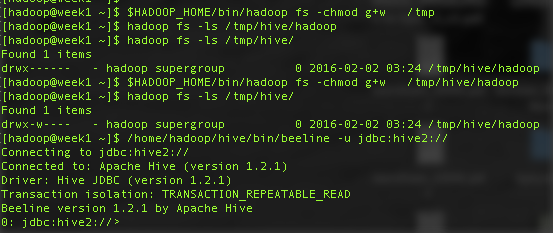
\includegraphics[scale=0.37]{fix_perm.png}
\centering
\end{figure}\\
\subsection*{Hive Test Use Case}
Following the instructions for the test use case using MovieLens data, I created the table using Hive CLI (despite the earlier mention of deprecation, as it seems simpler to use). I then exited out of the Hive CLI and downloaded the MovieLens data.
\pagebreak
\begin{figure}[!h]
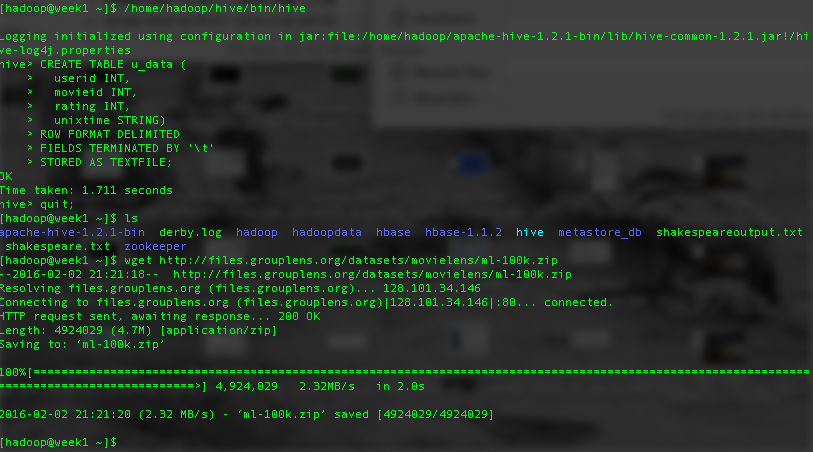
\includegraphics[scale=0.37]{create_table.png}
\centering
\end{figure}\\
\indent After the download, I tried to unpack the data but realized I needed to first go and grab the package for unzip as it was not installed. After getting it installed and unpacking the data, I was ready to load the data into the table using the \verb|LOAD DATA| function to load the u.data file. According to the README file, the u.data file is the "full u data set, 100000 ratings by 943 users on 1682 items".
\begin{figure}[!h]
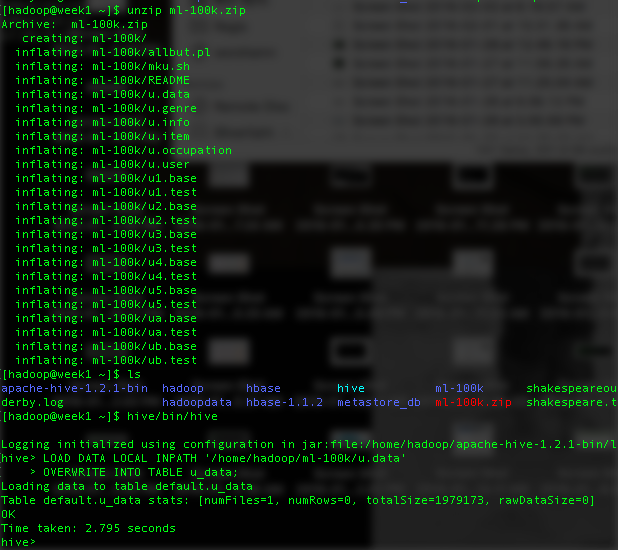
\includegraphics[scale=0.37]{load_udata.png}
\centering
\end{figure}\\
\indent Next I counted the rows in the table. Here I can see that it is running a mapreduce job to accomplish the task. I admit I was a little concerned this wasn't going to return anything because the previous step when I loaded the data in had a message about "numRows=0", but the query came back with the correct number of 100000.
\begin{figure}[!h]
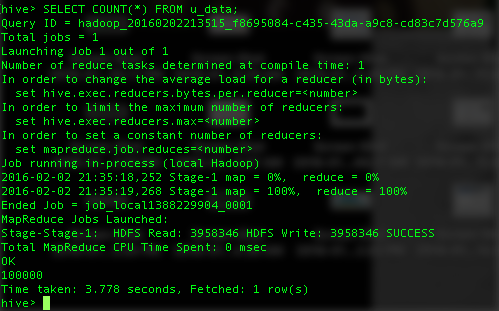
\includegraphics[scale=0.37]{count_rows.png}
\centering
\end{figure}\\
\indent Now the instructions were to make a python script for the "mapper script". I went ahead and created a scripts directory just for tidiness and built the script there. Looks like the script removes line endings, then segments out each line placing each part in a variable but most importantly the unixtime variable. It then takes that unixtime variable and converts it to a day of the week as a number (1-7) and then reformats the line back out again separated by tabs. Next I created another table and added the python script as a resource.
\begin{figure}[!h]
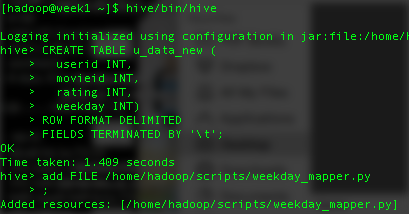
\includegraphics[scale=0.37]{add_file.png}
\centering
\end{figure}\\
\indent I ran the command that would "transform" the data from the original table to the data into the new table with the day of the week as a number. Though the thought did occur to me of why the exercise went to the the trouble of making another table instead of just adding a column with the converted days of the week value to the original table? After this completed I was then able to count from this data and \verb|GROUP BY| the day of the week.
\begin{figure}[!h]
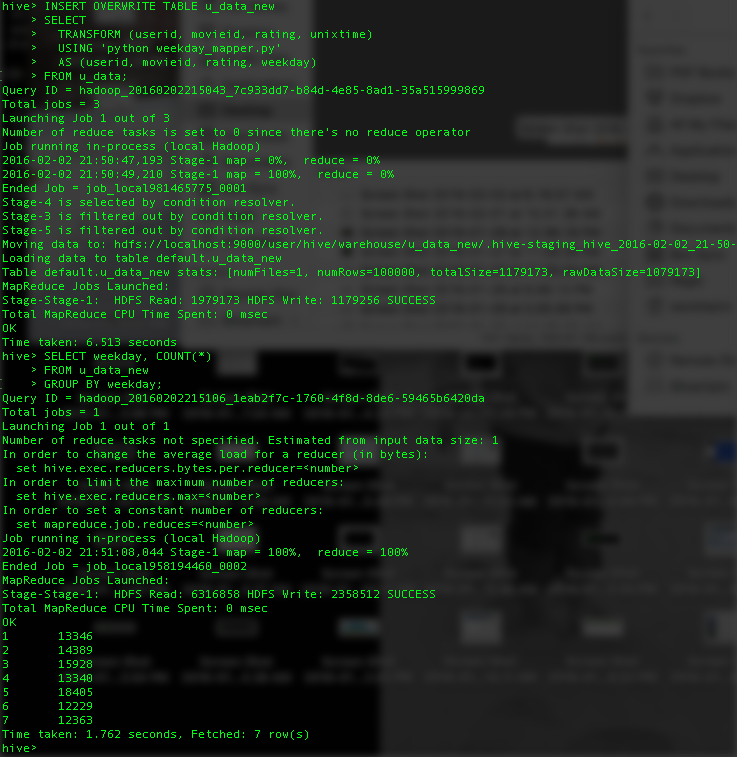
\includegraphics[scale=0.37]{final.png}
\centering
\end{figure}\\
\indent This shows that the most ratings happened on Fridays, followed by Wednesdays. Surprisingly, weekends were the least popular, but perhaps this is when the subjects watched the content in order to give it a review later in the week. Last I decided to try out some other HQL commands to show and describe the tables that now existed.
\pagebreak
\begin{figure}[!h]
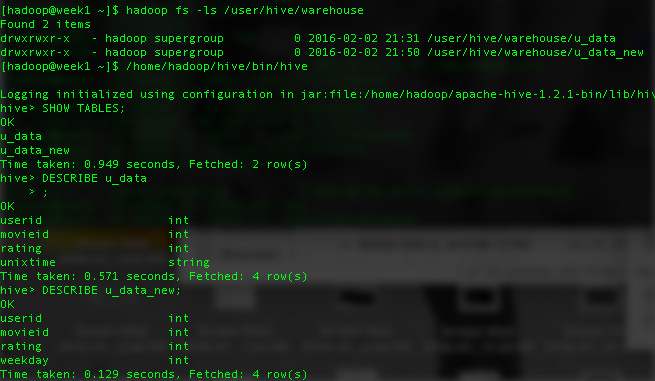
\includegraphics[scale=0.37]{explore01.png}
\centering
\end{figure}\\
\subsection*{References}
cwiki.apache.org, 2016. Retrieved from\\ https://cwiki.apache.org/confluence/display/Hive/GettingStarted\#GettingStarted-InstallingHivefromaStableRelease
\end{document}
